% !TEX program = xelatex
% Hand-edited seminar deck. build_content.py is the archived content generator.
% Metropolis theme vendored locally; format with python3 format_tex.py seminar.tex.
\documentclass[aspectratio=169,10pt]{beamer}
\usepackage{fontspec,amsmath,amssymb,booktabs,array,tikz,graphicx}
\usetheme[progressbar=frametitle,numbering=fraction,sectionpage=none,block=transparent]{metropolis}
\usetikzlibrary{positioning,arrows.meta}
\setsansfont{FiraSans}[Path=fonts/,Extension=.ttf,UprightFont=*-Regular,BoldFont=*-Bold,ItalicFont=*-Italic]
\setmainfont{FiraSans}[Path=fonts/,Extension=.ttf,UprightFont=*-Regular,BoldFont=*-Bold,ItalicFont=*-Italic]
\setmonofont{Menlo}[Scale=.8]
\definecolor{navy}{HTML}{23373B}
\definecolor{teal}{HTML}{168A85}
\definecolor{blue}{HTML}{2879B8}
\definecolor{purple}{HTML}{8154B8}
\definecolor{muted}{HTML}{68798B}
\definecolor{wash}{HTML}{EFF5F7}
\setbeamerfont{frametitle}{size=\large}
\setbeamerfont{block title}{size=\normalsize,series=\bfseries}
\setbeamerfont{block body}{size=\normalsize}
\setbeamersize{text margin left=.65cm,text margin right=.65cm}
\setlength{\parskip}{.1cm}
\makeatletter
\expandafter\patchcmd\csname beamer@@tmpl@title page\endcsname{\paperheight}{\dimexpr\paperheight-1cm\relax}{}{}
\makeatother
\renewcommand{\arraystretch}{1.12}
\newcolumntype{P}[1]{>{\raggedright\arraybackslash}p{#1}}
\title{Điều khiển đèn giao thông}
\subtitle{Mô phỏng GAMA và bốn phương pháp điều khiển}
\date{}
\hypersetup{colorlinks=true,urlcolor=blue,linkcolor=teal,pdftitle={Điều khiển đèn giao thông — Seminar}}
\begin{document}
  \begin{frame}[plain]
    \titlepage
  \end{frame}
  \begin{frame}{Đèn nên giữ xanh hay nhường hướng khác?}
    \relax
    \begin{block}{Bài toán}
      Khi nào nên chuyển đèn ở giao lộ ngã tư?
    \end{block}
    \begin{itemize}
      \item \textbf{Dựng môi trường:} đường, xe hỗn hợp, luật rẽ và nhập dòng.
      \item \textbf{Kết nối điều khiển:} GAMA trao đổi với Python; thử bốn phương pháp.
      \item \textbf{Kiểm chứng:} huấn luyện và so sánh trên cùng nhu cầu xe.
    \end{itemize}
    \vspace{.3cm}\alert{Mạch trình bày:} mô phỏng $\rightarrow$ quyết định $\rightarrow$ học $\rightarrow$ đánh giá.
  \end{frame}
  \begin{frame}{Môi trường: một ngã tư trong mạng nhiều tầng}
    \relax
    \begin{columns}[T,onlytextwidth]
      \begin{column}{.48\textwidth}{\centering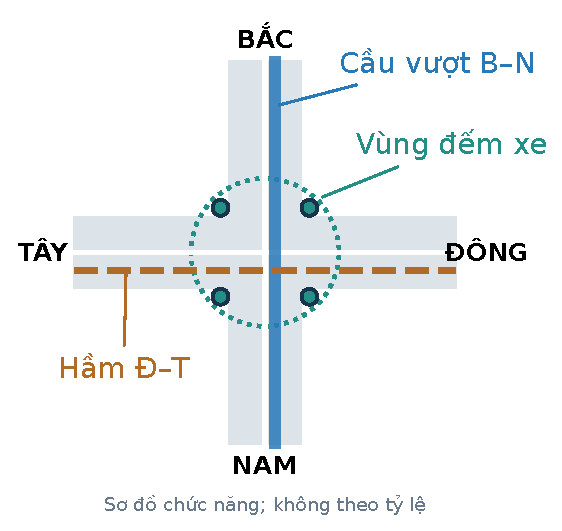
\includegraphics[width=\linewidth,height=4.65cm,keepaspectratio]{figures/network_map}\par}
      \end{column}
      \begin{column}{.48\textwidth}
        \begin{itemize}
          \item Không gian $2.000\times2.000$ m; bốn nhánh Bắc, Nam, Đông, Tây.
          \item \textbf{4 cột đèn × 2 nhóm} (thẳng/trái) = 8 nhóm tín hiệu.
          \item \textbf{1 bộ điều khiển trung tâm} phối hợp các hướng.
        \end{itemize}
      \end{column}
    \end{columns}
  \end{frame}
  \begin{frame}{Mỗi làn đường có 16 làn con}
    \relax
    {\centering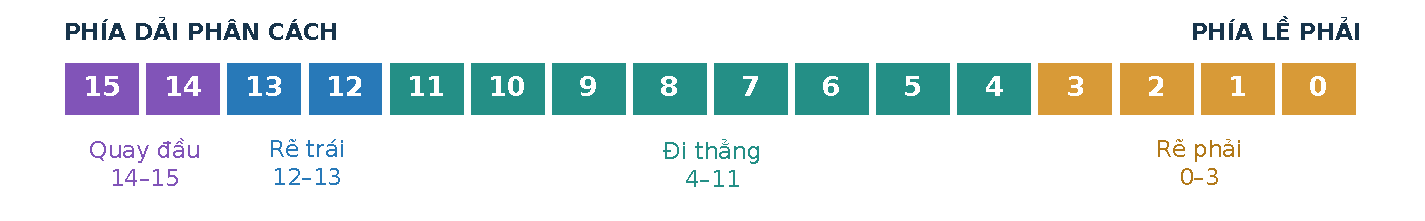
\includegraphics[width=\linewidth,height=2.0cm,keepaspectratio]{figures/sublanes}\par}
    \vspace{.25cm}
    \begin{center}
      \begin{minipage}{.78\linewidth}
        \begin{itemize}
          \item Mỗi làn con rộng \textbf{1,75 m}; bề rộng mô hình là 28 m/chiều.
          \item Xe máy chiếm 1 làn con; ô tô và buýt chiếm 2.
        \end{itemize}
      \end{minipage}
    \end{center}
  \end{frame}
  \begin{frame}{Xe chạy theo luật}
    \relax
    \begin{columns}[T,onlytextwidth]
      \begin{column}{.48\textwidth}
        \begin{block}{IDM làm gì?}
          Cứ mỗi 0,1 giây, mỗi xe tự hỏi: \emph{“Mình nên tăng ga, giữ nguyên hay đạp phanh?”}
        \end{block}
      \end{column}
      \begin{column}{.48\textwidth}
        \begin{block}{GAMA hỗ trợ sẵn}
          \begin{itemize}
            \item Khai báo \texttt{skills: [driving]} cho loài xe.
            \item Mỗi bước, reflex gọi \texttt{do drive}; driving skill tính bám xe bằng IDM.
          \end{itemize}
        \end{block}
      \end{column}
    \end{columns}
    \vspace{.3cm}
    \[
      a=a_{\max}\left[1-\left(\frac{v}{v_0}\right)^\delta-\left(\frac{s^*}{s}\right)^2\right]
    \]
  \end{frame}
  \begin{frame}{Lách và rẽ trái đều có điều kiện}
    \relax
    \begin{columns}[T,onlytextwidth]
      \begin{column}{.48\textwidth}
        \begin{block}{Đổi lane}
          \begin{itemize}
            \item Bộ lọc dự án kiểm tra khoảng trống trước/sau.
            \item GAMA áp dụng cơ chế MOBIL để xét đổi lane.
          \end{itemize}
        \end{block}
      \end{column}
      \begin{column}{.48\textwidth}
        \begin{block}{Đường rẽ trái Bézier}
          \begin{itemize}
            \item \textbf{Bậc 3 (cubic Bézier):} 4 điểm điều khiển $P_0,P_1,P_2,P_3$.
            \item Pha trái xanh và lối ra trống mới được vào.
          \end{itemize}
        \end{block}
      \end{column}
    \end{columns}
    \vspace{.1cm}
    \[
      B(t)=(1-t)^3P_0+3(1-t)^2tP_1+3(1-t)t^2P_2+t^3P_3,\quad t\in[0,1]
    \]
  \end{frame}
  \begin{frame}{AI được quyết định khi nào?}
    \relax
    \begin{columns}[T,onlytextwidth]
      \begin{column}{.48\textwidth}
        \begin{block}{Giới hạn của pha xanh}
          \begin{itemize}
            \item \textbf{Xanh tối thiểu 10 s} (\texttt{min\_green\_cycles} = 100): trong 10 s đầu AI chưa được quyết định.
            \item Tại 10, 15, 20, …, 55 s: hỏi lại sau mỗi 5 s.
          \end{itemize}
        \end{block}
      \end{column}
      \begin{column}{.48\textwidth}
        \begin{block}{Hai câu trả lời}
          \begin{itemize}
            \item \textbf{Giữ}: xanh thêm khoảng 5 s.
            \item \textbf{Chuyển}: vàng 3 s $\rightarrow$ trái 12 s $\rightarrow$ vàng 3 s $\rightarrow$ xanh trục kia.
            \item \textbf{Trần 60 s}: hệ thống ép chuyển nếu AI cứ giữ xanh.
          \end{itemize}
        \end{block}
      \end{column}
    \end{columns}
    \vspace{.3cm}
  \end{frame}
  \begin{frame}{Bốn phương pháp điều khiển}
    \relax
    \vspace{1cm}
    \begin{columns}[T,onlytextwidth]
      \begin{column}{.48\textwidth}
        \centering\Large Fixed-Time\par\vspace{1cm}Q-Learning
      \end{column}
      \begin{column}{.48\textwidth}
        \centering\Large Max-Pressure\par\vspace{1cm}Deep Q-Learning
      \end{column}
    \end{columns}
  \end{frame}
  \begin{frame}{Fixed-Time}
    \relax
    \begin{columns}[c,onlytextwidth]
      \begin{column}{.32\textwidth}
        \centering
        {\color{teal}\fontsize{46}{50}\selectfont\bfseries 30 s}\par
        \vspace{.1cm}
        \textbf{xanh thẳng cố định}
      \end{column}
      \begin{column}{.62\textwidth}
        \begin{block}{Quy tắc}
          Hết thời gian xanh, đèn chuyển theo lịch pha định sẵn. Số xe đang chờ không làm thay đổi thời điểm chuyển.
        \end{block}
      \end{column}
    \end{columns}
    \vspace{.65cm}
    \textbf{Một lượt chuyển pha}\par\vspace{.2cm}
    \begin{center}
      \begin{tikzpicture}[>=Latex,
        phase/.style={draw,rounded corners=3pt,minimum height=1.2cm,align=center,font=\small},
        every path/.style={draw=muted,->,thick}]
        \node[phase,draw=teal,fill=teal!10,minimum width=2.7cm] (green) {\textbf{Xanh thẳng}\\30 s};
        \node[phase,draw=orange,fill=orange!10,minimum width=1.55cm,right=.28cm of green] (yellow1) {\textbf{Vàng}\\3 s};
        \node[phase,draw=blue,fill=blue!10,minimum width=2.4cm,right=.28cm of yellow1] (left) {\textbf{Xanh trái}\\12 s};
        \node[phase,draw=orange,fill=orange!10,minimum width=1.55cm,right=.28cm of left] (yellow2) {\textbf{Vàng}\\3 s};
        \node[phase,draw=teal,fill=teal!10,minimum width=2.7cm,right=.28cm of yellow2] (next) {\textbf{Trục kia}\\xanh thẳng};
        \draw (green)--(yellow1);
        \draw (yellow1)--(left);
        \draw (left)--(yellow2);
        \draw (yellow2)--(next);
      \end{tikzpicture}
    \end{center}
  \end{frame}
  \begin{frame}{Max-Pressure}
    \relax
    \begin{center}
      {\Large\bfseries Áp lực đường nào lớn hơn thì ưu tiên bật đèn xanh hướng đó.}
    \end{center}
    \vspace{.1cm}
    \[
      P_j=(q_j+a_j)-d_j
    \]
    \begin{center}
      \small $q$: xe thẳng chờ · $a$: xe thẳng đang tới · $d$: xe phía thoát
    \end{center}
    \vspace{.35cm}
    \begin{center}
      \begin{tikzpicture}[
        pressure/.style={draw,rounded corners=3pt,minimum width=5.25cm,minimum height=1.55cm,align=center}]
        \node[pressure,draw=teal,fill=teal!10] (ns) {\textbf{Bắc–Nam}\\[.07cm]$(12+3)-4=\textcolor{teal}{\mathbf{11}}$};
        \node[pressure,draw=blue,fill=blue!10,right=.45cm of ns] (ew) {\textbf{Đông–Tây}\\[.07cm]$(4+2)-1=\textcolor{blue}{\mathbf{5}}$};
      \end{tikzpicture}
    \end{center}
    \vspace{.2cm}
    \begin{center}
      \textbf{Đông–Tây đang xanh:} $11>5+2$ $\Rightarrow$ chuyển sang Bắc–Nam.\\[.15cm]
      \small Ngưỡng 2 điểm giúp tránh chuyển pha khi chênh lệch quá nhỏ.
    \end{center}
  \end{frame}
  \begin{frame}{Reinforcement Learning - Học tăng cường}
    \relax
    \begin{center}
      \begin{tikzpicture}[node distance=.6cm, every node/.style={font=\normalsize}, b/.style={draw=teal,fill=wash,rounded corners,text width=2.5cm,align=center,minimum height=1.1cm}]
        \node[b] (s) {Quan sát\\\textbf{trạng thái $s$}};
        \node[b,right=of s] (a) {Chọn\\\textbf{hành động $a$}};
        \node[b,right=of a] (r) {Mô phỏng chạy\\\textbf{reward $r$}};
        \node[b,right=of r] (n) {Quan sát mới\\\textbf{trạng thái $s'$}};
        \draw[->,thick] (s)--(a);\draw[->,thick] (a)--(r);\draw[->,thick] (r)--(n);
      \end{tikzpicture}
    \end{center}
    \vspace{.4cm}
    \textbf{Tác tử học:} bộ điều khiển đèn. \quad \textbf{Môi trường:} ngã tư và các xe.\\[.3cm]
    \textbf{Chính sách:} quy tắc ánh xạ quan sát thành hành động.\\[.3cm]
    \textbf{Mục tiêu:} tăng tổng reward hiện tại và tương lai.
  \end{frame}
  \begin{frame}{Q-Learning: kinh nghiệm nằm trong bảng Q}
    \relax
    \begin{block}{}
      \textbf{Key:} sáu đặc trưng đã rời rạc hóa của tình huống giao thông.\\[.15cm]
      \textbf{Value:} hai điểm $[Q(\text{giữ xanh}),\,Q(\text{chuyển pha})]$.
    \end{block}
    \vspace{.15cm}
    \begin{center}
      \large $(2,0,1,0,0,1)\;\longrightarrow\;[-3,\,-8]$
    \end{center}
    \small Ví dụ minh họa: chọn \textbf{giữ xanh} vì $-3>-8$; Q là điểm lợi ích tương lai, không phải xác suất.
    \vspace{.2cm}
    \begin{itemize}
      \item Sáu đặc trưng cho tối đa $3\times3\times2\times2\times2\times3=\mathbf{216}$ key; chỉ tạo dòng khi gặp trong huấn luyện.
      \item File checkpoint \texttt{best\_q.pt} lưu dictionary \texttt{table} cùng trạng thái học khác. Đây là file nhị phân PyTorch, không phải bảng văn bản.
    \end{itemize}
    \small Sau mỗi trải nghiệm, thuật toán sửa điểm của hành động vừa chọn: $Q_{\rm mới}=Q_{\rm cũ}+0,1(\text{mục tiêu học}-Q_{\rm cũ})$.
  \end{frame}
  \begin{frame}{Sáu thành phần tạo nên một key của bảng Q}
    \relax
    \small
    \begin{tabular}{@{}P{3.15cm}P{1.7cm}P{7.9cm}@{}}
      \toprule
      Thành phần & Giá trị & Ý nghĩa tại lúc đèn ra quyết định\\
      \midrule
      $q_{\text{thẳng mình}}$ & 0 / 1 / 2 & Xe thẳng đang dừng ở trục xanh: 0 / 1–4 / từ 5 xe.\\
      $q_{\text{thẳng kia}}$ & 0 / 1 / 2 & Xe thẳng đang dừng ở trục còn lại: cùng ba mức.\\
      $\text{trái mình}$ & 0 / 1 & Trục xanh không / có xe đang chờ rẽ trái.\\
      $\text{trái kia}$ & 0 / 1 & Trục kia không / có xe đang chờ rẽ trái.\\
      $\text{thoát nghẽn}$ & 0 / 1 & Lối ra của trục xanh có ít nhất 5 xe hay không.\\
      $\text{tuổi xanh}$ & 0 / 1 / 2 & Xanh đã chạy $<25$ s / 25 đến $<45$ s / từ 45 s.\\
      \bottomrule
    \end{tabular}
    \par
    \vspace{.25cm}
    \alert{Sáu thành phần trạng thái} kết hợp thành tối đa \textbf{216 tình huống}; mỗi tình huống có hai điểm hành động.
  \end{frame}
  \begin{frame}{DQN: nhìn toàn bộ vòng ra quyết định và học}
    \relax
    \centering
    \resizebox{\linewidth}{!}{%
      \begin{tikzpicture}[>=Latex,font=\footnotesize\sffamily,
        flow/.style={->,line width=1.1pt,draw=teal},
        feedback/.style={->,line width=.9pt,draw=purple},
        decision/.style={draw=teal,rounded corners=3pt,fill=wash,align=center,minimum height=1.0cm},
        learning/.style={draw=purple,rounded corners=3pt,fill=purple!5,align=center,minimum height=.95cm}]
        \node[text=teal,font=\bfseries\footnotesize] at (1.1,5.32) {QUYẾT ĐỊNH};
        \node[decision,text width=1.8cm] (input) at (1.1,4.15) {\textbf{11 số}\\trạng thái $s$};
        \foreach \j in {0,...,7} {
          \foreach \i in {0,...,7} {
            \fill[teal] (2.80+0.15*\i,3.62+0.15*\j) circle (.047cm);
            \fill[teal] (4.85+0.15*\i,3.62+0.15*\j) circle (.047cm);
          }
        }
        \node[align=center] at (3.33,5.15) {\textbf{Lớp ẩn 1}\\64 nút};
        \node[align=center] at (5.38,5.15) {\textbf{Lớp ẩn 2}\\64 nút};
        \node[decision,text width=1.6cm] (q) at (7.75,4.15) {\textbf{2 điểm Q}\\giữ / chuyển};
        \node[decision,text width=1.48cm] (action) at (10.0,4.15) {\textbf{Chọn}\\hành động $a$};
        \node[decision,text width=1.52cm] (gama) at (12.25,4.15) {\textbf{GAMA}\\chạy tiếp};
        \draw[flow] ([xshift=2pt]input.east)--(2.65,4.15);
        \draw[flow] (3.98,4.15)--(4.70,4.15);
        \draw[flow] (6.05,4.15)--(q.west);
        \draw[flow] (q.east)--(action.west);
        \draw[flow] (action.east)--(gama.west);
        \node[align=center,text=purple] (reward) at (12.25,2.75) {\textbf{Reward $r$, trạng thái $s'$}\\sau khi mô phỏng};
        \draw[feedback] (gama.south)--(reward.north);
        \node[text=purple,font=\bfseries\footnotesize] at (1.1,1.40) {HỌC};
        \node[learning,text width=2.2cm] (replay) at (10.35,1.35) {\textbf{Replay: lưu}\\{\scriptsize $(s,a,r,s',d,\Delta t)$}};
        \node[learning,text width=2.2cm] (loss) at (7.20,1.35) {\textbf{Target $y$ + loss}\\so với $Q(s,a)$};
        \node[learning,text width=2.8cm] (grad) at (3.55,1.35) {\textbf{Backprop + Adam}\\sửa trọng số $W,b$};
        \draw[feedback] (reward.south) |- (replay.east);
        \draw[feedback] (replay.west)--(loss.east);
        \draw[feedback] (loss.west)--(grad.east);
        \draw[feedback] (grad.north) -- (3.55,2.65) -| (3.33,3.47);
      \end{tikzpicture}%
    }
    \par\vspace{.12cm}
  \end{frame}
  \begin{frame}{Hàm thưởng: xe chờ lâu làm điểm giảm}
    \relax
    \begin{center}
      \begin{tikzpicture}[>=Latex,
        rewardstep/.style={draw=teal,fill=wash,rounded corners=3pt,text width=3.25cm,
          minimum height=1.8cm,align=center,font=\small}]
        \node[rewardstep] (run) {\textbf{1. Chạy tiếp}\\Tới lần quyết định đèn tiếp theo};
        \node[rewardstep,right=.55cm of run] (count) {\textbf{2. Đếm xe dừng}\\Mỗi 0,1 s, đếm xe chạy $<1$ km/h};
        \node[rewardstep,right=.55cm of count] (score) {\textbf{3. Tính điểm}\\Cộng số xe $\times$ thời gian dừng};
        \draw[->,thick,muted] (run)--(count);
        \draw[->,thick,muted] (count)--(score);
      \end{tikzpicture}
    \end{center}
    \vspace{.25cm}
    \begin{center}
      \colorbox{wash}{\parbox{.72\linewidth}{\centering\vspace{.15cm}
        \textbf{Đổi thành điểm thưởng âm}\par\vspace{.1cm}
        {\Large $\displaystyle r=-\frac{1}{50}\sum_k q_k\cdot0,1\,\mathrm{s}$}\par\vspace{.15cm}}}
    \end{center}
    \vspace{.15cm}
    \begin{center}
      \small $q_k$ là số xe gần như dừng trong toàn mạng tại bước $k$.\\[.1cm]
      Reward hiện chưa tính độ an toàn như TTC/PET.
    \end{center}
  \end{frame}
  \begin{frame}{Quá trình train diễn ra như thế nào?}
    \relax
    \begin{enumerate}
      \item \textbf{Chuẩn bị:} tạo 40 lịch yêu cầu xe khác nhau cho 40 lượt huấn luyện.
      \item \textbf{Chạy mô phỏng:} mỗi episode reset ngã tư, chạy 8.000 bước (800 s). Actor DQN và Q-Learning thay phiên điều khiển; khi học có lúc thử ngẫu nhiên.
      \item \textbf{Ghi trải nghiệm:} sau mỗi quyết định, lưu quan sát, hành động, điểm phạt, quan sát mới và thời gian đã trôi qua.
      \item \textbf{Học:} sau mỗi nhóm tối đa 4 episode, nhập trải nghiệm theo đúng thứ tự episode; cả bảng Q và mạng DQN cùng được cập nhật.
      \item \textbf{Chọn mô hình:} cứ 10 episode kiểm tra trên 2 seed validation; lưu bản có hàng đợi thấp nhất.
    \end{enumerate}
    \vspace{.15cm}
    \small Một episode là một lượt chạy; trong lượt có nhiều quyết định và nhiều lần cập nhật.
  \end{frame}
  \begin{frame}{Đánh giá bằng những lượt chưa dùng để học}
    \relax
    \begin{tabular}{@{}P{2.5cm}P{3.5cm}P{6.2cm}@{}}
      \toprule
      Tập & Quy mô & Vai trò\\
      \midrule
      Train & 40 seed: 1001–1040 & Sửa bảng Q và trọng số DQN\\
      Validation & 3001–3002, mỗi 10 episode & Chọn checkpoint có hàng đợi thấp nhất\\
      Test & 5001–5005 × 4 phương pháp & Đánh giá chính sách đã đóng băng\\
      \bottomrule
    \end{tabular}
    \par
    \vspace{.4cm}
    \begin{itemize}
      \item Cùng yêu cầu xe, thời gian mô phỏng, lịch pha và luật di chuyển.
      \item Chọn mô hình bằng validation; giữ test cho đánh giá cuối.
      \item Khi test: giữ nguyên mô hình, không học thêm hoặc thử ngẫu nhiên.
    \end{itemize}
  \end{frame}
  \begin{frame}{Benchmark: bốn phương pháp, sáu chỉ số (1/2)}
    \relax
    {\normalsize\setlength{\tabcolsep}{3pt}
    \begin{tabular}{@{}P{4.0cm}*{4}{>{\centering\arraybackslash}p{2.45cm}}@{}}
      \toprule
      Trung bình 5 seed & Fixed-Time & Max-Pressure & Q-Learning & DQN\\
      \midrule
      Số lượng xe thông qua & 228,6 & 232,4 & 238,8 & \textbf{243,6}\\
      Số lượng xe dừng trung bình & 24,17 & 17,23 & 13,23 & \textbf{12,65}\\
      Thời gian xe chờ (s) & 292,79 & 289,85 & 287,82 & \textbf{286,97}\\
      \bottomrule
    \end{tabular}
    \par}
    \vspace{.35cm}
  \end{frame}
  \begin{frame}{Benchmark: bốn phương pháp, sáu chỉ số (2/2)}
    \relax
    {\normalsize\setlength{\tabcolsep}{3pt}
    \begin{tabular}{@{}P{4.0cm}*{4}{>{\centering\arraybackslash}p{2.45cm}}@{}}
      \toprule
      Trung bình 5 seed & Fixed-Time & Max-Pressure & Q-Learning & DQN\\
      \midrule
      Yêu cầu còn ngoài mạng & 1.045,0 & \textbf{1.043,8} & 1.045,4 & 1.044,4\\
      Hành trình xe đã hoàn thành (s) & 277,27 & \textbf{264,64} & 268,83 & 268,23\\
      Thời gian chờ trong mạng lớn nhất (s) & 555,08 & 552,72 & 497,22 & \textbf{439,62}\\
      \bottomrule
    \end{tabular}
    \par}
    \vspace{.35cm}
  \end{frame}
  \begin{frame}{Ngoài ùn tắc, mô phỏng còn đo rủi ro}
    \relax
    \small
    \begin{tabular}{@{}P{2.3cm}P{10.3cm}@{}}
      \toprule
      Chỉ số & Mô hình đang ghi nhận gì?\\
      \midrule
      TTC & Thời gian dự kiến tới va chạm nếu giữ vận tốc; đếm mẫu có TTC $<1$ s.\\
      TIT & Cộng mức TTC thấp hơn ngưỡng an toàn theo từng bước 0,1 s.\\
      PET & Khoảng thời gian từ khi xe trước rời ô xung đột tới khi xe sau vào; đếm PET $<1,5$ s.\\
      DRAC & Mức giảm tốc cần để tránh xe trước, $\Delta v^2/(2g)$; lưu giá trị lớn nhất.\\
      Phanh gấp & Đếm mẫu có gia tốc $<-3,4$ m/s$^2$; phanh rất mạnh $<-5,0$ m/s$^2$.\\
      \bottomrule
    \end{tabular}
    \par
    \vspace{.2cm}
    Trong DRAC, $g$ là khoảng hở và $\Delta v$ là tốc độ tiếp cận.\par
    \vspace{.2cm}
  \end{frame}
\end{document}
